When the user hits the Run button, and assuming the results are
successful. The results are presented here.  A successful run or
download of a job that ran successfully will result in 3 tabbed
widgets being displayed in this panel.  The first panel shows summary
statistics: mean and stdDev values or min-max values if discrete set,
i.e. multiple events for each of the EDP's specified in the EDP panel.

\begin{figure}[!htbp]
  \centering {
    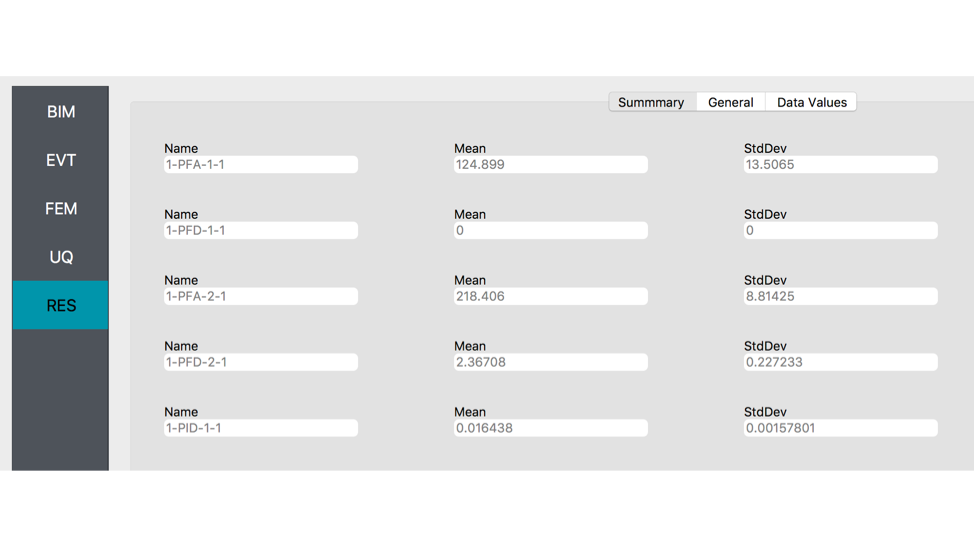
\includegraphics[width=0.8\textwidth]
    {figs/Figure12.png} }
  \caption{RES}
  \label{fig:figure12}
\end{figure}

The second panel shows the summary information.

\begin{figure}[!htbp]
  \centering {
    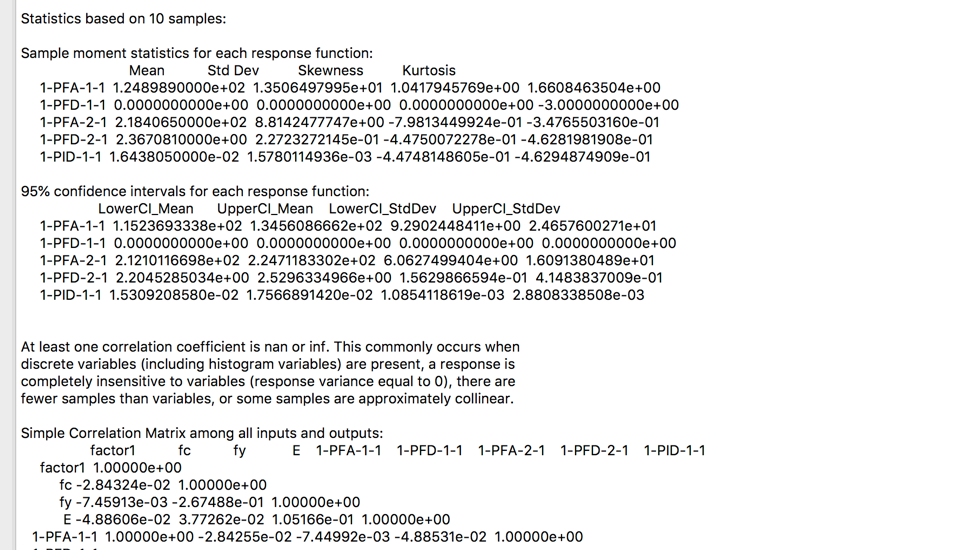
\includegraphics[width=0.8\textwidth]
    {figs/Figure13.png} }
  \caption{RES General tab}
  \label{fig:figure13}
\end{figure}

The third panel presents graphically and in tabular form the
results. By selecting different columns with left and right mouse
buttons in the table below the graphic, the information in the graph
is changed. Selecting the left mouse button changes the Y axis, the
right mouse changes the X axis. If the same column is selected using
both left and right keys, the CDF and PDF is displayed. If last mouse
press was with the left button, the PDF and if right the CDF.
 
As for the columns. You will see a column for each random variable the
workflow came across. There may be more than you specified if the
applications want the UQ engine to consider their own variables in the
computation. The outputs at present are limited to:

\begin{figure}[!htbp]
  \centering {
    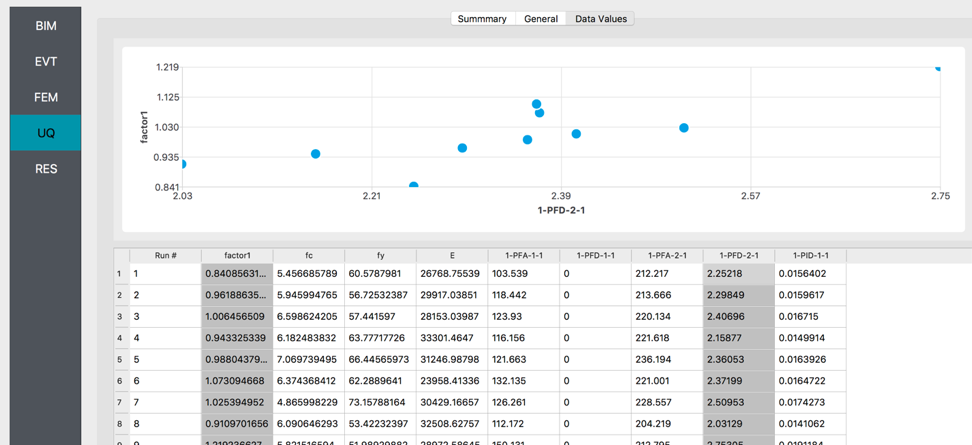
\includegraphics[width=0.8\textwidth]
    {figs/Figure14.png} }
  \caption{UQ Data Values}
  \label{fig:figure14}
\end{figure}
